\chapter{Analisis}
\label{chap:analisis}

Pada bab ini akan dijelaskan mengenai analisis grafik dari data sensor-sensor pada \textit{smartphone} ketika sedang mengangguk dan menggeleng, analisis aplikasi-aplikasi sejenis, dan analisis metode pendeteksi gerakan kepala. 

\section{Analisis Aplikasi Sejenis}
\label{sec:analisis_aplikasi_sejenis}

Aplikasi sejenis pada perangkat \textit{Virtual Reality} Google Cardboard hanyalah ada satu aplikasi saja. Aplikasi tersebut adalah aplikasi InMind VR. Aplikasi sejenis pada perangkat \textit{Virtual Reality} Oculust Rift adalah Trial of the Rift Drifter dengan Asunder yang di kembangkan oleh AldinDynamics \cite{aldin_dynamics}. Aplikasi sejenis pada \textit{Virtual Reality} Oculust Rift tidak dapat dianalisis karena penulis tidak memiliki perangkat Oculust Rift. \\

\textbf{Analisis InMind VR}\\

InMind VR merupakan permainan \textit{Virtual Reality} yang seakan-akan pengguna berada dalam sel-sel otak seorang manusia. Permainan ini dimainkan dengan mengarahkan arah pandang kepala ke arah sel-sel neuron yang dapat menyebabkan gangguan mental (Gambar \ref{fig:screenshot_inmind_task}). Akan ada 50 sel neuron yang dapat menyebabkan gangguan mental. Sel-sel yang dapat menyebabkan gangguan mental adalah sel-sel yang berwarna merah seperti pada Gambar \ref{fig:screenshot_inmind_gameplay}.

\begin{figure}[htbp]
\centering
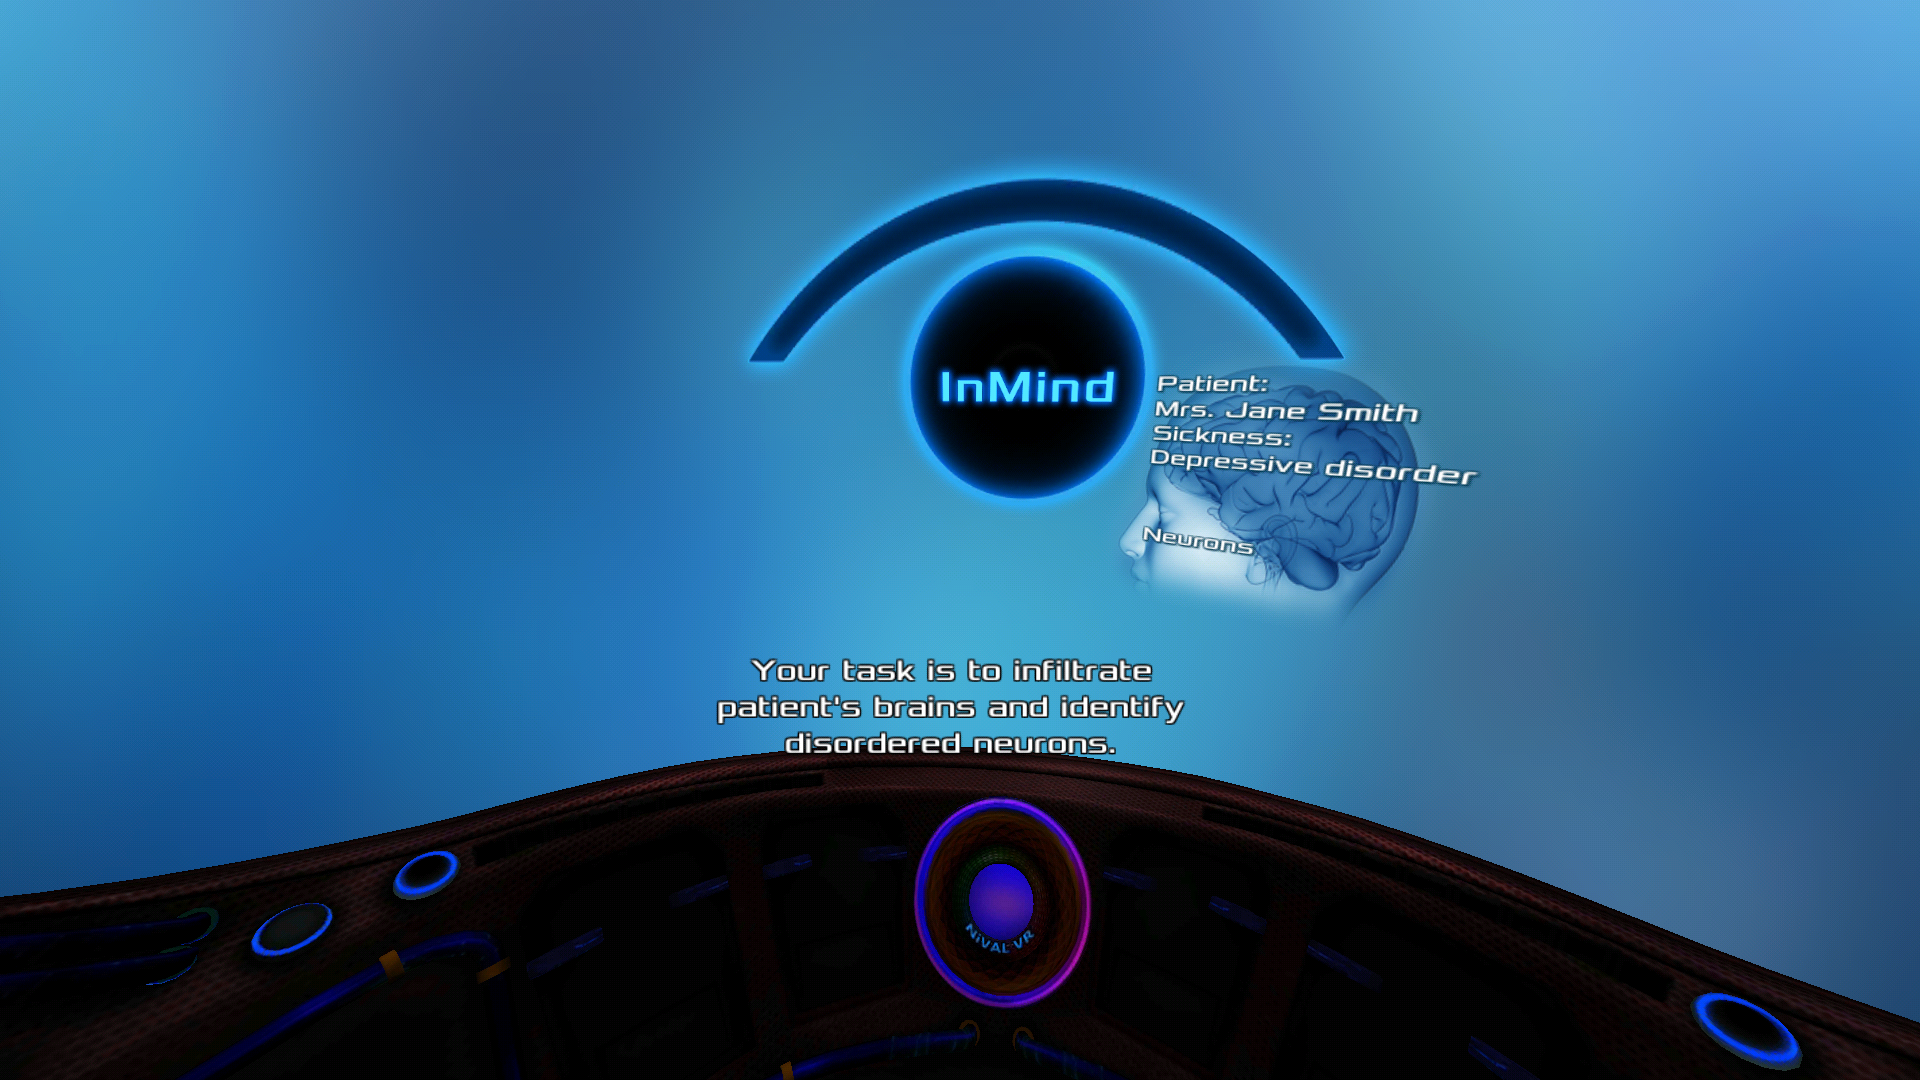
\includegraphics[scale=0.6]{Gambar/screenshot-inmind-task.png}
\caption{\textit{Screenshot} task yang diberikan aplikasi InMind VR.}
\label{fig:screenshot_inmind_task}
\end{figure}

Pada permulaan permainan pengguna diberi pertanyaan apakah pengguna sudah siap untuk melakukan permainan tersebut seperti yang ditunjukkan pada Gambar \ref{fig:screenshot_inmind_nod}.

\begin{figure}[htbp]
\centering
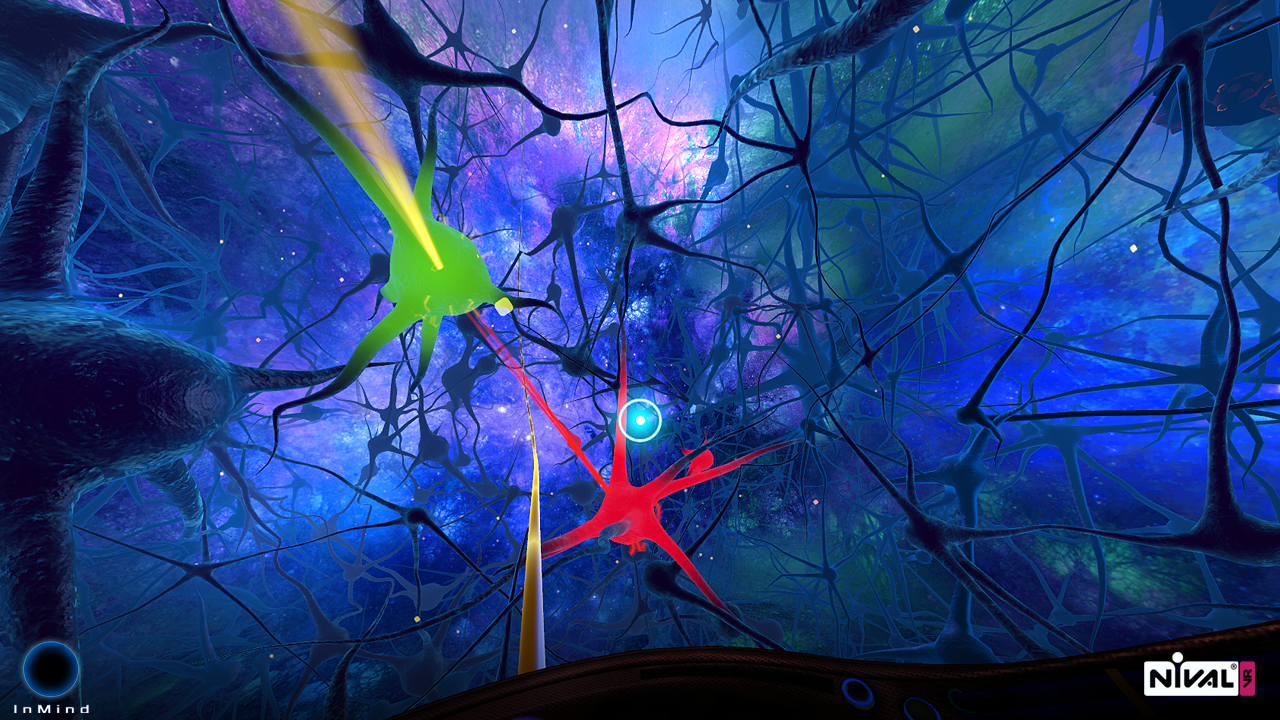
\includegraphics[scale=0.7]{Gambar/screenshot-inmind-gameplay.jpg}
\caption{\textit{Screenshot} aplikasi InMind VR ketika permainan berlangsung.}
\label{fig:screenshot_inmind_gameplay}
\end{figure}

Analisis dilakukan dengan cara mengetes aplikasi ini dengan mengangguk dan menggeleng yang spesifik. Mengangguk dilakukan dengan cara-cara berikut:
\begin{enumerate}
	\item Mengangguk secara pelan.
	\item Mengangguk yang diawali dengan gerakan ke atas.
	\item Melihat kebawah saja tanpa membalikkan kepala ke posisi semula.
	\item Tidak menggerakkan kepala sama sekali.
\end{enumerate}

Dari keempat percobaan mengangguk yang dilakukan, hanya percobaan pertama dengan percobaan ketiga yang terdeteksi mengangguk. Aplikasi ini dapat disimpulkan dengan hanya menggerakkan kepala kebawah saja sudah dapat dianggap mengangguk oleh aplikasi ini. Pada percobaan kedua dan keempat terjadi keganjilan dari pendeteksian anggukkan. Pada percobaan kedua dan keempat aplikasi tetap akan melanjutkan permainan setelah beberapa detik berlalu. Sel-sel yang dapat menyebabkan gangguan mental adalah sel-sel yang berwarna merah seperti pada Gambar \ref{fig:screenshot_inmind_gameplay}. 

Ketika dilakukan percobaan menggeleng, tidak ada respon apapun dari aplikasi ini. Aplikasi ini akan tetap melanjutkan ke permainan setelah beberapa detik telah berlalu. Hal tersebut menyimpulkan bahwa aplikasi ini tidak dapat mendeteksi gerakan menggeleng. Oleh karena itu hal yang dilakukan oleh aplikasi ini hanyalah melihat apakah pengguna sudah melihat kebawah atau belum saja.

\begin{figure}[htbp]
\centering
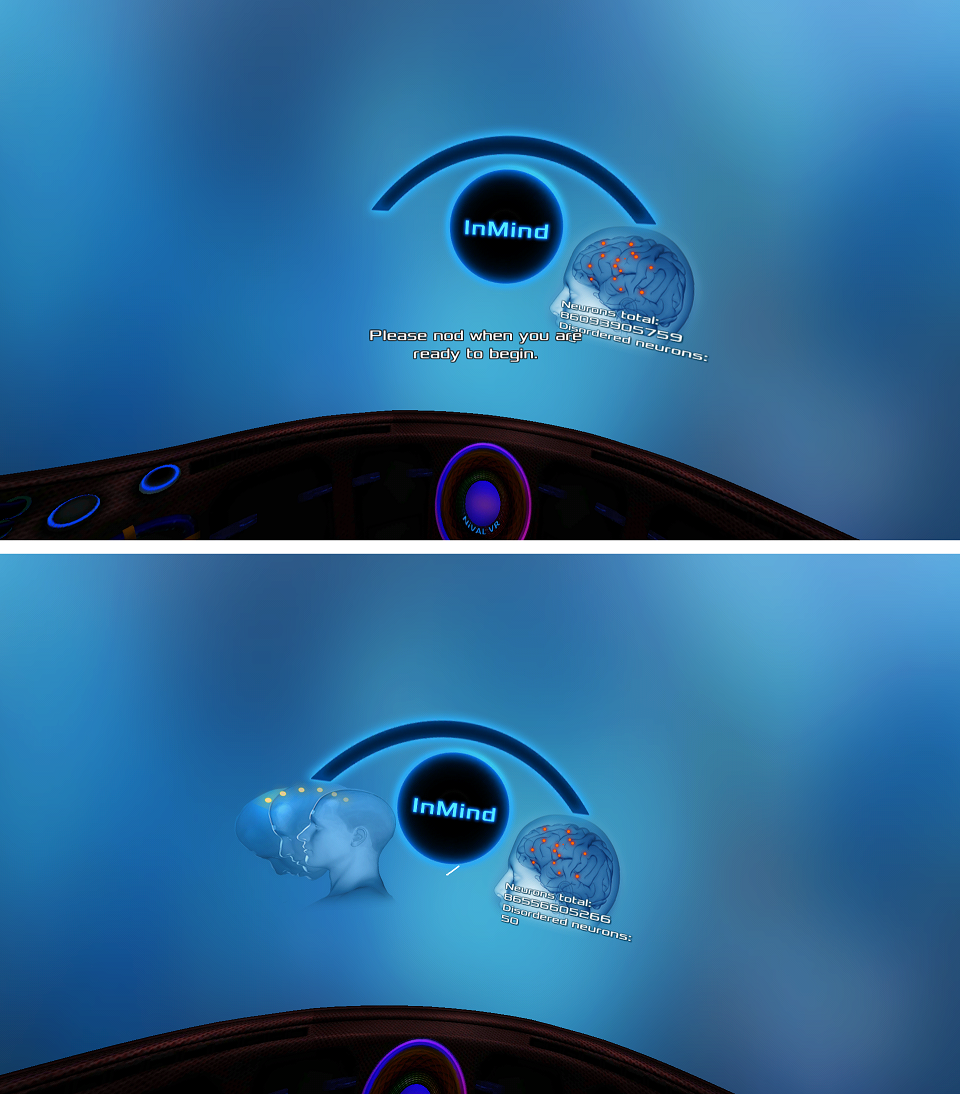
\includegraphics[scale=0.6]{Gambar/screenshot-inmind-nod.png}
\caption{\textit{Screenshot} aplikasi InMind VR ketika meminta pengguna untuk mengangguk jika telah siap.}
\label{fig:screenshot_inmind_nod}
\end{figure}



\section{Perekaman Data Sensor}
\label{sec:perekaman_data_sensor}

Pada analisis ini akan dilakukan perekaman mengganguk dan menggeleng dengan sensor-sensor pada Android. Perekaman-perekaman ini akan dilakukan pada tiga kondisi muka pengguna. Kondisi muka yang pertama adalah kondisi muka pengguna ketika menghadap ke depan, digambarkan dengan Gambar \ref{fig:posisi-muka} bagian (a). Kondisi muka yang kedua adalah kondisi muka pengguna keita menghadap ke atas sekitar $45^{\circ}$ dari pandangan muka menghadap ke atas digambarkan dengan Gambar \ref{fig:posisi-muka} bagian (b). Kondisi muka yang ketiga adalah kondisi muka ketika menghadap serong ke kiri atas digambarkan dengan Gambar \ref{fig:posisi-muka} bagian (c). Anggukan yang dilakukan oleh pengguna hanya sebanyak satu kali mengangguk ke bawah saja. Sedangkan dalam menggeleng akan bergerak ke kiri terlebih dahulu dan ke kanan setelahnya dan diakhiri pada posisi muka kembali ke posisi awal.

\begin{figure}[htbp]
\centering
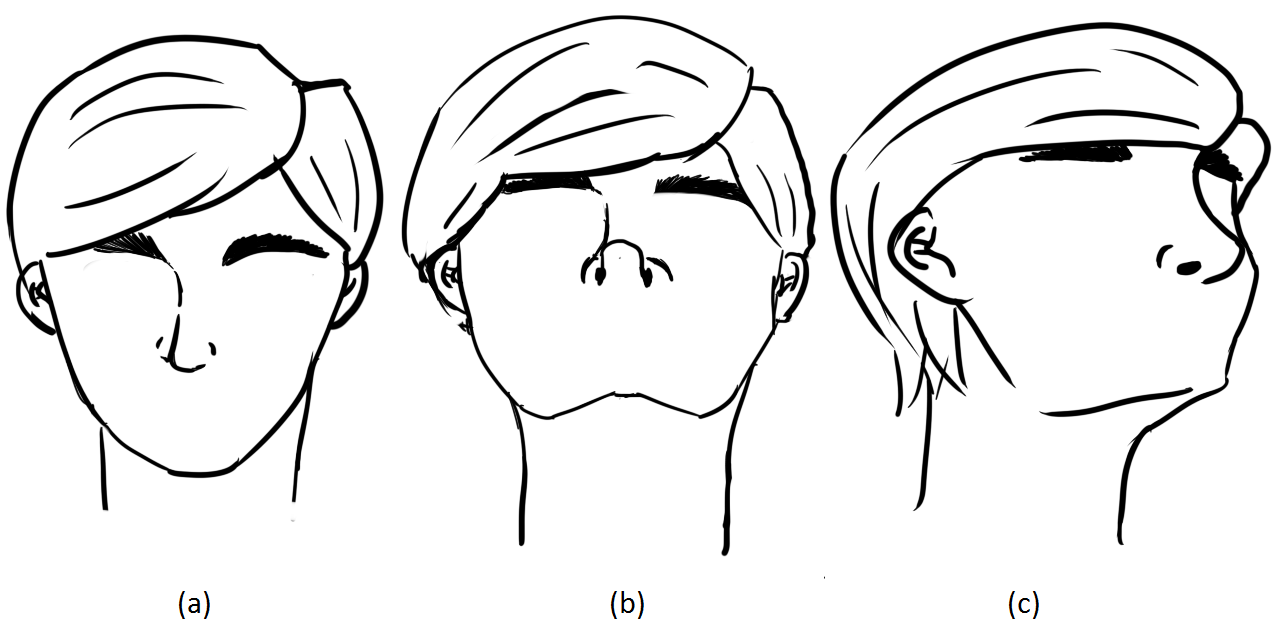
\includegraphics[scale=0.4]{Gambar/posisi-muka.png}
\caption{Gambar untuk mendeskripsikan posisi dari muka sebelum melakukan gerakan menggeleng atau mengangguk. Gambar (a) adalah kondisi muka ketika sedang menghadap ke depan. Gambar (b) adalah kondisi muka ketika sedang menghadap ke atas. Gambar(c) adalah kondisi muka ketika sedang menghadap ke serong kiri atas.}
\label{fig:posisi-muka}
\end{figure}

Grafik-grafik yang akan ditunjukkan pada bab ini akan memiliki beberapa karakteristik. Sumbu y pada grafik yang akan ditunjukkan akan merepresentasikan besar nilainya, Sedangkan sumbu x akan merepresentasikan waktunya. Grafik yang ditunjukkan akan memiliki beberapa nilai, tergantung dari jumlah nilai yang dikembalikan untuk setiap sensornya. Contohnya pada sensor \textit{accelerometer} yang memiliki tiga jenis nilai, sehingga pada grafik akan terbentuk tiga buah garis nilai. Aplikasi akan merekam beberapa sensor secara langsung ketika pengguna mengangguk atau menggeleng, sehingga nilai wakunya akan sama untuk kondisi muka yang sama walaupun sensornya berbeda.

Analisis grafik data sensor-sensor pada Android dilakukan dengan membuat suatu aplikasi perekam sensor-sensor yang ada pada \textit{smartphone} Android terlebih dahulu. Aplikasi ini akan merekam nilai-nilai yang dihasilkan dari sebagian sensor-sensor pada android setiap ada perubahan. Pada skripsi ini, nilai sensor-sensor yang dibutuhkan adalah sensor \textit{accelerometer}, \textit{gyroscope}, \textit{rotation vector}, dan \textit{geomagnetic rotation}. Aplikasi menyimpan nilai sensor-sensor menggunakan format CSV \textit{(Comma Separated Values)}. Dari data yang diperoleh oleh apliasi tersebut dibuatkan grafiknya menggunakan aplikasi Microsoft Excel. Penjelasan dari setiap grafik akan dijelaskan pada subbab-subbab berikut.
\subsection{Perekaman Grafik Sensor \textit{Accelerometer}}
\label{sec:analisis_grafik_sensor_accelerometer}
Seperti yang sudah dijelaskan pada bab sebelumnya, sensor \textit{accelerometer} akan mendeteksi seluruh percepatan yang terjadi pada perangkat Android. Perekaman ini perangkat android akan diletakkan di depan muka pengguna, sehingga percepatan yang mempengaruhi perangkat Android hanya percepatan gravitasi dengan percepatan yang dilakukan oleh gerakan kepala pengguna. 

\begin{figure}[htbp]
\centering
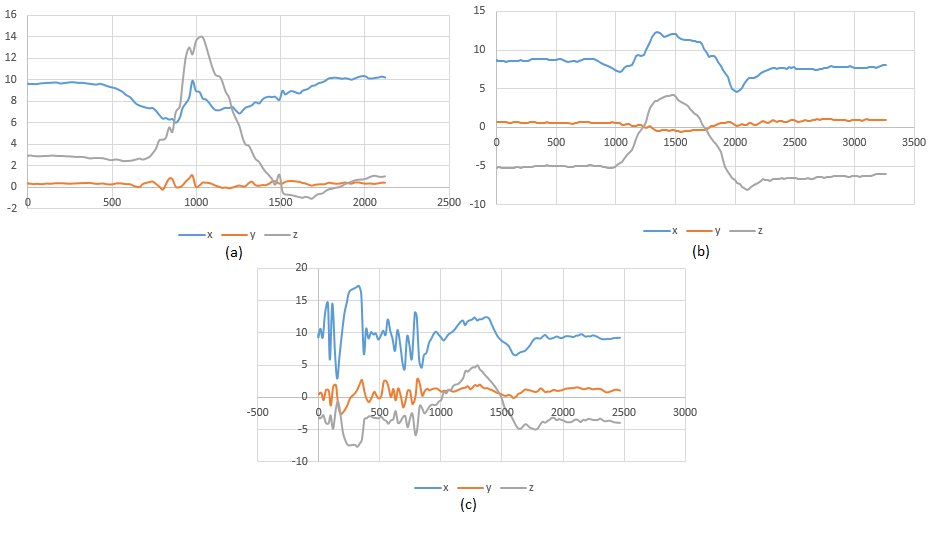
\includegraphics[scale=0.6]{Gambar/grafik-sensor-accelerometer-mengangguk.png}
\caption{Grafik nilai kuaternion dari sensor \textit{accelerometer} ketika pengguna mengangguk dengan posisi muka awal (a) menghadap ke depan, (b) menghadap ke atas, (c) menghadap ke kiri atas.} 
\label{fig:grafik-sensor-accelerometer-mengangguk}
\end{figure}

Gambar \ref{fig:grafik-sensor-accelerometer-mengangguk} merupakan grafik-grafik yang terbentuk dari nilai yang di terima oleh sensor \textit{accelerometer} ketika pengguna sedang mengangguk. Pada Gambar \ref{fig:grafik-sensor-accelerometer-mengangguk} grafik (a) terlihat nilai z menaik dan nilai x menurun ketika sedang mengangguk. Tetapi nilai x kembali menaik ketika nilai z sudah hampir mencapai nilai tertinggi. Sedangkan nilai y terlihat cukup konstan di sekitar angka 0. Pada grafik (b) terlihat nilai x dengan y memiliki pola yang serupa ketika mengangguk. Kedua nilai menaik ketika pengguna sedang mengangguk. Nilai x bermulai dari nilai sekitar sebesar 9 sedangkan nilai z bernilai sekitar sebesar -5. Sama seperti pada grafik (a) nilai y terlihat konstan di sekitar angka 0. Selanjutnya grafik (c) pada Gambar \ref{fig:grafik-sensor-accelerometer-mengangguk} merupakan grafik yang terbentuk dari nilai yang diterima oleh sensor \textit{accelerometer} ketika pengguna mengangguk dan sedang menghadap ke kiri atas. Grafik pada bagian ini sangat tidak beraturan. Pada Grafik ini sulit untuk membedakan kondisi kapan pengguna sedang mengangguk. Goncangan yang terjadi terhadap \textit{smartphone}, seperti munculnya notifikasi mungkin dapat menyebabkan hal ini. Namun pada waktu mencapai 1000 milidetik terlihat cukup stabil. Pada grafik (c) di Gambar \ref{fig:grafik-sensor-accelerometer-mengangguk} juga menunjukkan bahwa nilai x dengan z memiliki pola yang sama hingga akhir, dan nilai y konstan di sekitar angka 0. Hasil nilai tersebut serupa dengan kasus ketika menghadap ke atas. 


\begin{figure}[htbp]
\centering
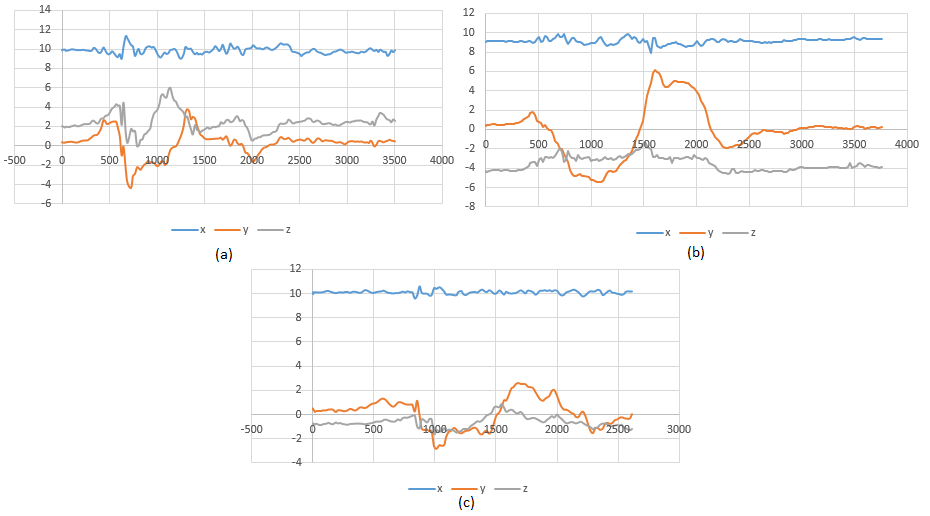
\includegraphics[scale=0.6]{Gambar/grafik-sensor-accelerometer-menggeleng.png}
\caption{Grafik nilai kuaternion dari sensor \textit{accelerometer} ketika pengguna menggeleng dengan posisi muka awal (a) menghadap ke depan, (b) menghadap ke atas, (c) menghadap ke kiri atas.} 
\label{fig:grafik-sensor-accelerometer-menggeleng}
\end{figure}

Gambar \ref{fig:grafik-sensor-accelerometer-menggeleng} merupakan grafik yang terbentuk dari nilai yang diterima oleh sensor \textit{accelerometer} ketika pengguna menggeleng. Pada grafik (a), nilai x konstan di sekitar angka 10. Nilai y dengan z pada grafik (a) menaik dan menurun ketika pengguna menggelengkan kepala. Pada grafik (b) nilai x terlihat konstan di sekitar nilai 10 dan nilai z sedikit tidak beraturan di sekitar nilai -4 hingga -2. Nilai y mengalami kenaikan dan penurunan saat menggeleng. Pada grafik (c) di Gambar \ref{fig:grafik-sensor-accelerometer-menggeleng} nilai x konstan di sekitar nilai 10. Nilai y menaik dan menurun, tetapi tidak beraturan. Nilai pada z juga mengalami sedikit kenaikan dan penurunan. Pada grafik (b) dengan (c) nilai z mengalami perubahan yang tidak beraturan dan puncak tertinggi dengan puncak terendahnya tidak terlalu berbeda jauh dengan nilai awalnya.

Dari keenam grafik tersebut terlihat bahwa nilai yang terpengaruh ketika pengguna sedang mengangguk adalah nilai x dengan z. Nilai y tidak berpengaruh karena nilai y cenderung konstan. Nilai yang terpengaruh ketika pengguna sedang menggeleng adalah nilai y. Nilai x terlihat konstan pada setiap grafik, tetapi nilai z mengalami sedikit pergerakan ketika pengguna sedang mengangguk sehingga tidak dapat dipastikan bahwa nilai z terpengaruhi gerakan menggeleng. 

\subsection{Perekaman Grafik Sensor \textit{Gyroscope}}
\label{sec:analisis_grafik_sensor_gyroscope}
Perekaman menggunakan sensor \textit{gyroscope} akan mendapatkan percepatan angular yang terjadi setiap waktunya. Berbeda dengan sensor \textit{accelerometer} yang dapat terpengaruhi oleh lingkungan sekitar seperti gravitasi dan percepatan lainnya, sensor ini hanya akan merekam perputaran yang terjadi pada perangkat saja. Hal ini sangat menguntungkan dalam mendeteksi suatu gerakan karena tidak harus memperdulikan kasus dari pengaruh luar. 


\begin{figure}[htbp]
\centering
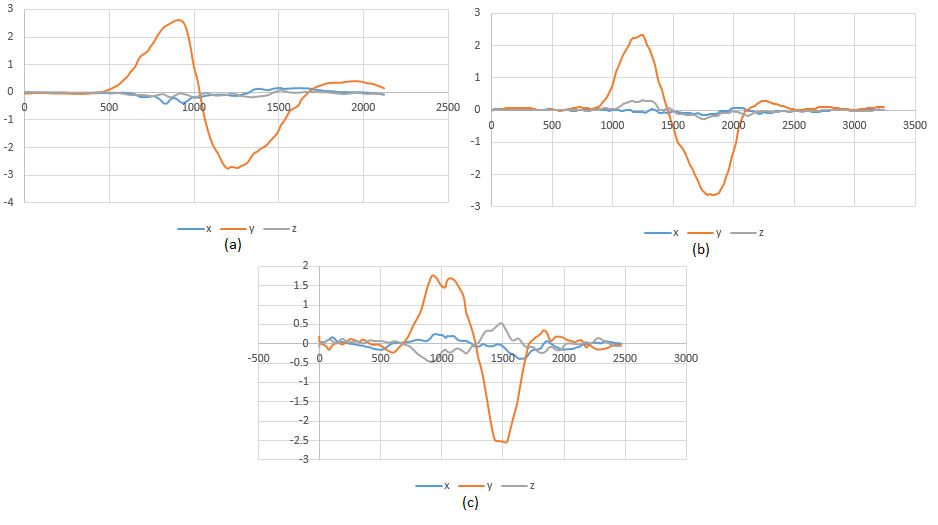
\includegraphics[scale=0.6]{Gambar/grafik-sensor-gyroscope-mengangguk.png}
\caption{Gambar grafik nilai sensor \textit{gyroscope} ketika pengguna mengangguk dengan posisi muka awal (a) menghadap ke depan, (b) menghadap ke atas, (c) menghadap ke kiri atas.}
\label{fig:grafik-sensor-gyroscope-mengangguk}
\end{figure}
Gambar \ref{fig:grafik-sensor-gyroscope-mengangguk} menunjukkan nilai-nilai sensor \textit{gyroscope} ketika pengguna sedang mengangguk. Grafik (a) membentuk sebuah bukit dan lembah pada nilai y. Bukit yang terjadi disini menunjukkan ketika pengguna menggerakan kepalanya kebawah, dan ketika kepala pengguna kembali ke posisi semula percepatan angularnya berbalik arah sehingga menimbulkan lembah. Nilai x dengan z cenderung bernilai 0. Grafik (b) mirip seperti grafik pada Gambar \ref{fig:grafik-sensor-gyroscope-mengangguk}. Begitu pula pada grafik (c) yang memiliki pola yang serupa dengan yang grafik-grafik sebelumnya.

\begin{figure}[htbp]
\centering
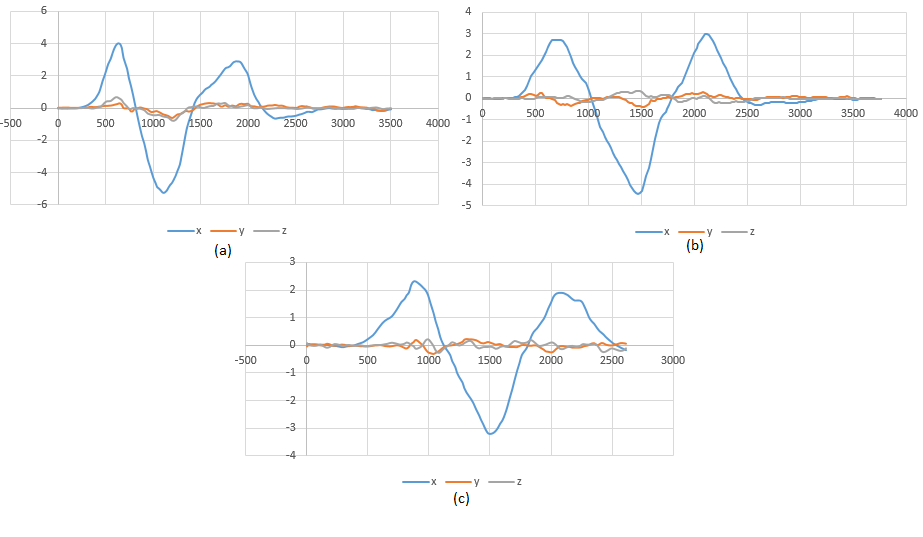
\includegraphics[scale=0.6]{Gambar/grafik-sensor-gyroscope-menggeleng.png}
\caption{Gambar grafik nilai sensor \textit{gyroscope} ketika pengguna menggeleng dengan posisi muka awal (a) menghadap ke depan, (b) menghadap ke atas, (c) menghadap ke kiri atas.} 
\label{fig:grafik-sensor-gyroscope-menggeleng}
\end{figure}

Gambar \ref{fig:grafik-sensor-gyroscope-menggeleng} menunjukkan nilai-nilai sensor \textit{gyroscope} ketika pengguna sedang menggeleng. Pada grafik (a) nilai yang mengalami kenaikan dan penurunan adalah nilai x dan nilai-nilai lainnya cenderung berada pada nilai 0. Nilai x membentuk 2 buah bukit dan 1 buah lembah. Bukit pertama terjadi ketika pengguna menggerakan kepalanya ke kiri. Lembah pertama terjadi ketika pengguna menggerakan kepalanya ke kanan. Bukit kedua terjadi ketika pengguna menggerakan kepalanya kembali ke posisi semula. Pada grafik (b) dengan grafik (c) menunjukkan pola grafik yang serupa dengan grafik pada Gambar (a).

Dari hasil-hasil tersebut dapat disimpulkan bahwa arah pandang pengguna tidak mempengaruhi sensor \textit{gyroscope} dalam mendeteksi gerakan kepala. Nilai-nilai yang dikembalikan oleh sensor \textit{gyroscope} memiliki  pola grafik yang jauh lebih rapih dibandingkan grafik-grafik yang dihasilkan oleh sensor \textit{accelerometer}. Selain itu sensor gyroscope hanya menggunakan 1 jenis nilai yang dipengaruhi oleh pergerakan kepala, sedangkan accelerometer ada 2 jenis nilai yang di pengaruhi gerakan kepala pada saat mengangguk. Oleh karena itu sensor gryoscope lebih baik dalam mendeteksi gerakan yang terjadi pada perangkat android.

\subsection{Perekaman Grafik Sensor \textit{Rotation Vector}}
\label{sec:analisis_grafik_sensor_rotation_vector}

Perekaman menggunakan sensor \textit{rotation vector} akan mendapatkan sebuah kuaternion yang merepresentasikan perputaran yang terjadi pada perangkat Android. Perputaran ini akan dideskripsikan dengan suatu vektor sebagai sumbu putarnya dan sudut perputarannya. Berbeda dengan sensor \textit{gyroscope} yang merekam kecepatan perputaran yang terjadi pada suatu waktu, sensor \textit{rotation vector} akan mengembalikan nilai kuaternion untuk mendefinisikan suatu kondisi putaran pada saat itu. 

\begin{figure}[htbp]
\centering
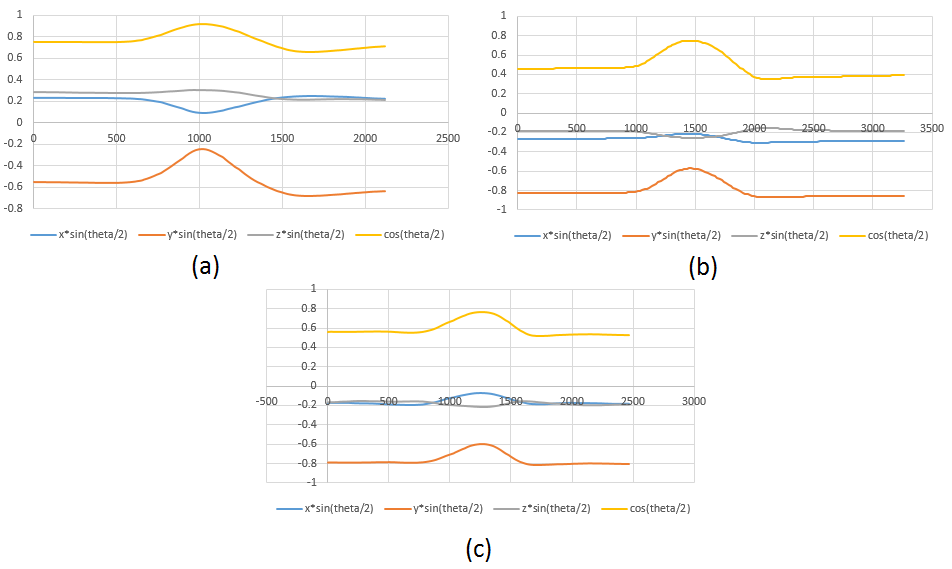
\includegraphics[scale=0.6]{Gambar/grafik-sensor-rot-vector-mengangguk.png}
\caption{Grafik nilai kuaternion dari sensor \textit{rotation vector} ketika pengguna mengangguk dengan posisi muka awal (a) menghadap ke depan, (b) menghadap ke atas, (c) menghadap ke kiri atas.} 
\label{fig:grafik-sensor-rot-vector-mengangguk}
\end{figure}

Gambar \ref{fig:grafik-sensor-rot-vector-mengangguk} menunjukkan nilai-nilai sensor \textit{rotation vector} ketika pengguna sedang mengangguk. Pada grafik (a) terbentuk sebuah bukit pada garis berwarna jingga dengan kuning, dan lembah pada garis berwarna biru. Garis yang berwarna abu cenderung stabil di angka 0.3. Grafik (b) menunjukkan pola yang mirip pada bagian (a) namun berbeda nilainya saja. Pada grafik (a) garis berwarna kuning dimulai pada angka sekitar 0.7, sedangkan pada grafik (b) garis berwarna jingga dimulai pada angka sekitar 0.4. Garis biru pada grafik ini tidak membentuk sebuat lembah seperti  pada grafik pada grafik (a). Garis berwarna abu cenderung konstan pada nilai -0.2, sedangkan pada grafik (a) cenderung konstan di sekitar 0.3. Garis berwarna jingga memiliki pola yang sama dengan garis berwarna kuning, hanya berbeda pada nilainya saja. Seperti pada grafik-grafik sebelumnya, grafik (c) ini memiliki pola yang sama dengan grafik lainnya. Grafik ini juga hanya nilainya saja yang berbeda dengan grafik lainnya. Kemiripan pola ini memungkinkan mempermudah pendeteksian gerakan kepala. 

\begin{figure}[htbp]
\centering
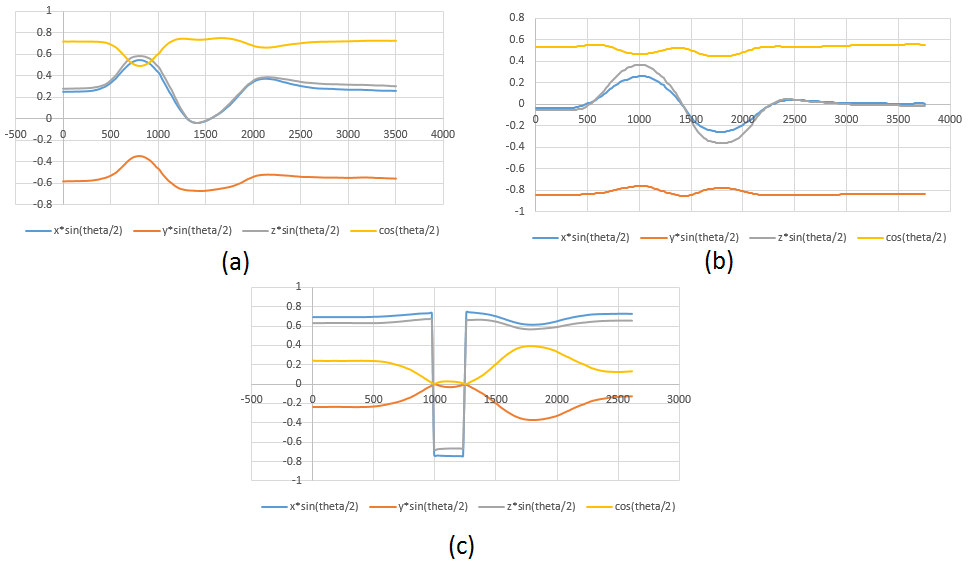
\includegraphics[scale=0.6]{Gambar/grafik-sensor-rot-vector-menggeleng.png}
\caption{Grafik nilai kuaternion dari sensor \textit{rotation vector} ketika pengguna menggeleng dengan posisi muka awal (a) menghadap ke depan, (b) menghadap ke atas, (c) menghadap ke kiri atas.} 
\label{fig:grafik-sensor-rot-vector-menggeleng}
\end{figure}

Gambar \ref{fig:grafik-sensor-rot-vector-menggeleng} menunjukkan nilai-nilai sensor \textit{rotation vector} ketika pengguna sedang menggeleng. Pada grafik (a) terbentuk sebuh bukit yang diikuti dengan lembah pada garis berwarna biru dengan abu-abu. Garis berwarna kuning membentuk suatu lembah yang setelahnya cenderung konstan. Berbeda pada garis kuning yang membentuk bukit kemudian setelahnya cenderung konstan. Grafik (b) memiliki kemiripan dengan grafik (a), garis biru dengan garis abu-abu memiliki pola yang sama yaitu membentuk bukit dengan lembah ketika pengguna menggelengkan kepala. Garis kuning dengan jingga cenderung konstan, berbeda dengan grafik (a) yang membentuk bukit atau lembah. Pada grafik (c) garis-garis membentuk suatu pola yang tidak normal. Garis kuning membentuk sebuah lembah, tetapi membentuk suatu bukit kecil ketika nilainya mencapai nilai 0 pada milidetik ke 1000. Garis jingga memiliki pola yang berlawanan dengan garis kuning. Pada saat garis kuning dengan garis jingga mencapai angka 0 perubahan drastis pun terjadi pada garis biru dengan abu-abu. Pada milidetik ke 1000 garis biru dengan abu mengalami perubahan nilai yang sangat drastis. Kedua nilai tersebut berubah dari nilai yang berkisar diantara 0.6 sampai 0.7 menjadi berkisar diantara -0.7 sampai -0.8. Kasus ini tidak berarti sensor sedang mengalami kegagalan akurasi (\textit{accuracy fail}), tetapi memang seperti itulah karakteristik dari perputaran menggunakan kuaternion pada android. Perputaran yang terjadi pada batas mendekati sebelum terjadinya dengan setelah perubahan nilai yang drastis memiliki hasil perputaran yang sama. Hal ini disebabkan karena melakukan perputaran dengan vektor sebagai sumbu dapat memiliki 2 buah nilai yang sejenis. Dua buah nilai tersebut akan menghasilkan perputaran yang sama ketika arah vektor dengan arah putarnya di balikkan seperti yang ditunjukkan pada Gambar \ref{fig:penjelasan-perputaran-quaternion-android-sensor}. Sepertinya pada sistem android nilai $\cos (theta/2)$ didesain agar tidak bernilai negatif, sehingga nilai-nilai yang lainnya akan mengalami perubahan nilai yang drastis ketika nilai $\cos (theta/2)$ mencapai angka 0.


\begin{figure}[htbp]
\centering
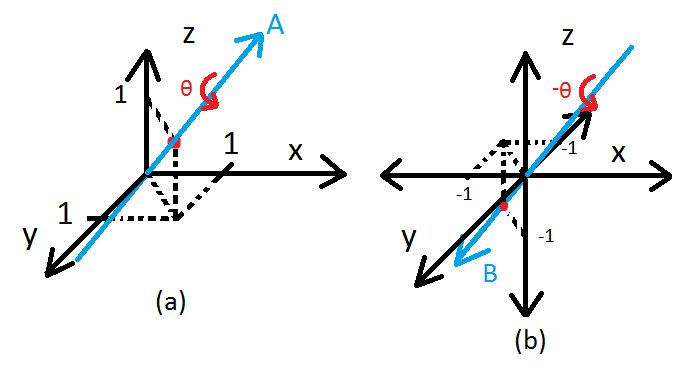
\includegraphics[scale=0.6]{Gambar/penjelasan-perputaran-quaternion-android-sensor.png}
\caption{Dua buah rotasi yang identik dengan nilai kuaternion yang berbeda.} 
\label{fig:penjelasan-perputaran-quaternion-android-sensor}
\end{figure}

\section{Analisis Data Sensor untuk Mendeteksi Gerakan Kepala}

Dari ketiga hasil pecobaan pada sensor-sensor pada bab \ref{sec:perekaman_data_sensor} dapat disimpulkan bahwa sensor \textit{gyroscope} adalah sensor yang terbaik untuk mendeteksi gerakan kepala. Data dari sensor \textit{accelerometer} akan susah untuk digunakan dalam mendeteksi gerakan kepala karena terganggu dengan aktivitas-aktivitas diluar gerakan pengguna yang juga ikut terekam oleh sensor \textit{accelerometer}. Data dari sensor \textit{rotation vector} juga akan lebih rumit dibandingkan sensor \textit{gyroscope}. Hal ini karena perputaran yang di rekam oleh sensor \textit{rotation vector} merekam kondisi putar pada suatu saat. Hasil rekaman ini akan mempersulit pada saat pendeteksian gerakan kepala karena harus melakukan proses untuk menghitung kecepatan kepala bergerak, agar dapat membedakan gerakan mengangguk atau menggeleng atau sekedar menoleh biasa. 
Dalam mendeteksi gerakan mengangguk dengan menggeleng banyak batas-batas yang perlu diperhatikan. Batas-batas tersebut untuk mengetahui apakah pengguna benar-benar mengangguk atau menggeleng atau sekedar menoleh biasa. Batas-batas yang perlu diperhatikan adalah:

\begin{itemize}
	\item Kecepatan pengguna menoleh.
	\item Jarak waktu pada saat pengguna melakukan melawan arah gerakan.
	\item Simpangan terbesar kepala saat mengangguk atau menggeleng.
\end{itemize}

Kecepatan pengguna menjadi batas karena gerakan kepala yang kecepatannya cenderung pelan biasanya bukan merupakan gerakan mengangguk ataupun menggeleng. Kecepatan ini dapat langsung diperoleh menggunakan sensor \textit{gyroscope}. Kecepatan yang dibutuhkan adalah kecepatan perputaran maksimum yang dilakukan oleh pengguna. Kecepatan maksimum dapat diperoleh dengan mengambil nilai puncak tertinggi dengan terendah. Jika nilai puncaknya mencapai kecepatan tertentu, gerakan tersebut dapat diperkirakan merupakan gerakan mengangguk ataupun menggeleng.

Gerakan menggeleng atau mengangguk biasanya memiliki selang waktu yang sangat sempit, karena pengguna biasanya langsung melawan arah secara langsung ketika sedang mengangguk ataupun menggeleng. Nilai ini dapat diperoleh dengan menghitung jarak antara bukit dengan lembah yang terbentuk pada grafik seperti yang dijelaskan pada Gambar \ref{fig:grafik-penjelasan-jarak-waktu-melawan-gerakan}. Idealnya gerakan menggeleng tidak memiliki rentang waktu ini, namun mungkin sebagian orang masih menghasilkan rentang waktu yang cukup sedikit. Oleh karena itu mungkin batas waktu yang ditentukan di sini adalah sekitar 100 milidetik. Jika rentang waktunya melebihi batas waktu tersebut, maka gerakan tersebut mungkin bukan merupakan gerakan mengangguk ataupun gerakan menggeleng. 

\begin{figure}[htbp]
\centering
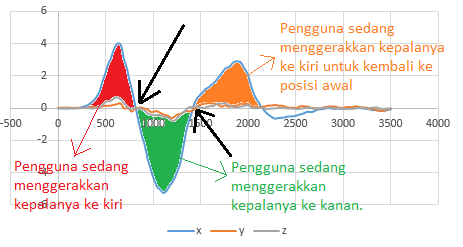
\includegraphics[scale=0.6]{Gambar/grafik-penjelasan-jarak-waktu-melawan-gerakan.png}
\caption{Deskripsi grafik pada saat pengguna menggeleng. Yang ditunjuk oleh panah berwarna hitam adalah selang waktu yang terjadi saat pengguna melawan arah gerakan kepala.} 
\label{fig:grafik-penjelasan-jarak-waktu-melawan-gerakan}
\end{figure}

Simpangan terbesar ini juga penting untuk dijadikan batasan-batasan dalam mendeteksi gerakan mengangguk ataupun menggeleng. Simpangan kepala yang sangat kecil dapat diragukan untuk dianggap sebagai gerakan mengangguk atau menggeleng. Simpangan ini dapat diperoleh dengan menghitung luas yang dibentuk dari bukit atau lembah yang terbentuk pada grafik. Contoh pada Gambar \ref{fig:grafik-penjelasan-jarak-waktu-melawan-gerakan} simpangan terbesar yang terjadi ketika pengguna menggerakkan kepalanya pertama kali ke kiri adalah luas pada bidang yang diarsir merah. Simpangan terbesar yang terjadi ketika pengguna menggerakaan kepalanya ke kanan adalah luas bidang yang diarsir berwarna hijau dikurangi dengan luas pada bidang yang diarsir merah. Pengurangan ini dilakukan karena luas bidang yang diarsir berwarna hijau merupakan simpangan yang terjadi setelah kepala sudah menghadap ke kiri. Begitu pula dengan luas bidang yang diarsir berwarna jingga yang akan dikurangi dengan hasil pengurangan luas sebelumnya.

\section{Analisis Metode Pendeteksi Gerakan Kepala}

Seperti yang sudah dijelaskan pada bab \ref{sec:android_sensor_framework}, data akan didapatkan setiap ada perubahan nilai pada sensor dengan rentang waktu tertentu, bergantung dengan konfigurasinya. Pendeteksian ini membutuhkan data yang \textit{real-time}, sehingga akan lebih baik jika menggunakan konfigurasi kecepatan pengambilan data setiap 20.000 mikrodetik. Penggunaan konfigurasi dengan kecepatan 0.000 mikrodetik tidak terlalu baik, karena akan menggunakan kemampuan processor yang sangat tinggi.

\subsection{Algoritma Mendeteksi Gerakan Mengangguk}
\label{ssec:algoritma_mendeteksi_gerakan_mengangguk}

Algoritma akan dipanggil setiap kali ada perubahan nilai dari sensor. Algoritma ini akan menyimpan nilai-nilai batas-batas yang telah didefinisikan, luas yang terbentuk dari lembah dan bukit terakhir, waktu mulai dan berakhirnya suatu bukit atau lembah. Algoritma ini akan di panggil secara berulang-ulang hingga menghasilkan hasil yang benar. Data akan disimpan pada attribut, agar setiap pemanggilan dapat mendapatkan data dari pemanggilan sebelumnya. 

Berikut adalah keterangan dari data-data yang disimpan pada attribut:
\begin{itemize}
	\item \texttt{passLimitUp}, attribut ini akan mencatat apakah pengguna sudah melewati batas kecepatan sudut ketika kepala pengguna bergerak ke atas.
	\item \texttt{passLimitDown}, attribut ini akan mencatat apakah pengguna sudah melewati batas kecepatan sudut ketika kepala pengguna bergerak ke bawah.
	\item \texttt{currentlyLimitUp}, attribut ini akan menunjukkan bahwa pada saat ini gerakan pengguna sedang bergerak ke atas dan melebihi batas kecepatan sudutnya.
	\item \texttt{currentlyLimitDown}, attribut ini akan menunjukkan bahwa pada saat ini gerakan pengguna sedang bergerak ke bawah dan melebihi batas kecepatan sudutnya.
	\item \texttt{angSpeedLimit}, attribut ini akan menyimpan batas kecepatan sudut.
	\item \texttt{lastYAngSpeed}, attribut ini akan memiliki kecepatan sudut Y pada pemanggillan method sebelumnya. 
	\item \texttt{lastT}, attribut ini akan memiliki waktu dipanggilnya method sebelumnya. 
	\item \texttt{calcArea}, attribut ini akan menyimpan besar luas bukit atau, lembah yang terjadi. Luas bukit akan bernilai positif, dan nilai lembah akan bernilai negatif. 
	\item \texttt{startTValley}, attribut ini akan menyimpan waktu mulai lembah yang memenuhi syarat kecepatan sudut minimal. 
	\item \texttt{endTValley}, attribut ini akan menyimpan waktu akhir lembah yang memenuhi syarat kecepatan sudut minimal.
	\item \texttt{startTCurrMotion}, attribut ini akan menyimpan waktu mulai suatu gerakan(bukit atau lembah) yang sedang berlangsung sekarang.
	\item \texttt{endTCurrMotion}, attribut ini akan menyimpan waktu akhir suatu gerakan(bukit atau lembah) yang sedang berlangsung sekarang.
	\item \texttt{deviationLimit} adalah batas simpangan untuk melakukan gerakan mengangguk.
	\item \texttt{deviationMotionDown}, attribut ini akan menyimpan simpangan yang terjadi ketika pengguna menggeraka kepalanya ke bawah. 
	\item \texttt{deviationMotioUp}, attribut ini akan menyimpan simpangan yang terjadi ketika pengguna menggeraka kepalanya ke atas. 
\end{itemize}
\begin{algorithm}
	\caption{Nod Detection Algoritm}
	\label{alg:algoritma-pendeteksi-gerakan-mengangguk}
	\begin{algorithmic}[1]
	\Function{detectNod}{$yAngSpeed$}
		\State $currT \gets $current Time 
		\If {$yAngSpeed > angSpeedLimit$}
			\State $passLimitUp \gets true$
			\State $currPassLimitUp \gets true$
		\ElsIf {$yAngSpeed < angSpeedLimit * -1$}
			\State $passLimitDown \gets true$
			\State $currPassLimitDown \gets true$
		\EndIf
		\If {X values intersect with x(time) axis}
			\State $xIntersect \gets ((-lastYAngSpeed / (yAngSpeed - lastYAngSpeed)) * (currT - lastT))+lastT$
			\State $endTCurrMotion \gets xIntersect$
			\State $areaBeforeIntersect \gets ((xIntersect - lastT) / 1000) * lastYAngSpeed / 2$
			\State $calcArea \gets calcArea + areaBeforeIntersect$
			\If {$currPassLimitDown$}
				\State $startTValley \gets startTCurrMotion$
				\State $endTValley \gets endTCurrMotion$
				\State $deviationMotionDown \gets calcArea$
				\If {$deviationMotionDown < deviationLimit * -1$}
					\State $passLimitDownDeviation \gets true$
				\EndIf
			\ElsIf {$currPassLimitUp$}
				\State $waktuMulaiBukit \gets startTCurrMotion$
				\State $waktuAkhirBukit \gets endTCurrMotion$
				\State $deviationMotionUp = calcArea$
				\If {$deviationMotionUp > deviationLimit$}
					\State $passLimitUpDeviation \gets true$
				\EndIf
			\EndIf
			\State $calcArea \gets 0$
			\State $areaAfterIntersect \gets ((currT - xIntersect) / 1000) * yAngSpeed / 2$ 
			\State $calcArea \gets calcArea + areaAfterIntersect$ 
			\State $startTCurrMotion \gets xIntersect$ 
			\State $currPassLimitDown \gets false$ 
			\State $currPassLimitUp \gets false$ 
		\Else 
			\State $calcArea \gets calcArea + ((lastYAngSpeed + yAngSpeed) / 1000) * (currT - lastT) / 2$
		\EndIf
		\State $lastYAngSpeed \gets yAngSpeed$
		\State $lastT \gets currT$
		
		\If {hill and valley time values has been set \textbf{AND} all condition have been met}
			\Return $true$
		\Else
			\Return $false$
		\EndIf
	\EndFunction  
	\end{algorithmic}
\end{algorithm}

Algoritma \ref{alg:algoritma-pendeteksi-gerakan-mengangguk} akan mengembalikan nilai true jika pengguna sedang mengangguk. Baris ke-2 hingga baris ke-8 adalah untuk mengecek kecepatan putar sekarang, apakah sudah melampaui batas yang ditentukan atau belum. Untuk mengetahui titik potong secara akurat dapat menggunakan rumus persamaan garis dari dua buah titik yang dinotasikan dengan Notasi \ref{eq:persamaan-garis-dua-titik}.   

\begin{equation}
		\frac{y-y_1}{y_2-y_1} = \frac{x-x_1}{x_2-x_1} \\
\label{eq:persamaan-garis-dua-titik}
\end{equation}
dengan,
\[
	\begin{split}
		y_1 = & lastYAngSpeed\\
		y_2 = & yAngSpeed\\
		x_1 = & lastT\\
		x_2 = & currT
	\end{split}
\]

Notasi \ref{eq:persamaan-garis-dua-titik} dijabarkan sesuai dengan penjabaran \ref{eq:aljabar-pencarian-titik-potong} sehingga menjadi rumus yang berada pada algoritma \ref{alg:algoritma-pendeteksi-gerakan-mengangguk} baris ke-10. Nilai titik potong x ini juga menjadi indikator waktu untuk rentang waktu dari suatu bukit atau lembah, yang akan digunakan untuk mendapatkan jarak waktu pada saat pengguna melawan arah gerakan. Baris ke-14 hingga ke-25 pada algoritma \ref{alg:algoritma-pendeteksi-gerakan-mengangguk} adalah untk mengecek apakah simpangan yang terjadinya sudah melewati batas yang ditetapkan atau belum dan mencatatnya ke dalam attribut \texttt{passLimitDownDeviation} atau \texttt{passLimitUpDeviation}. Pada baris ke-26 hingga ke-28 untuk memulai menghitung luas yang baru. Baris ke-32 dan baris ke-33 untuk menghitung luas ketika tidak berpotongan dengan sumbu x. Baris ke-36 untuk pengecekan jarak antara bukit dengan lembah dapat diselesaikan dengan mengurangi waktu mulai bukit dengan waktu akhir lembah. Sehingga hasil untuk mengecek apakah semua batas sudah terpenuhi dapat di selesaikan dengan operasi (AND) biasa. 

\begin{equation}
	\begin{split}
		y = & 0\\		
		\frac{0-y_1}{y_2-y_1} = & \frac{x-x_1}{} \\
		\frac{-y_1}{y_2-y_1} x_2-x_1 = & x-x_1 \\
		x = & (\frac{-y_1}{y_2-y_1} x_2-x_1) +x_1
	\end{split}
\label{eq:aljabar-pencarian-titik-potong}
\end{equation}


\subsection{Algoritma Mendeteksi Gerakan Menggeleng}
\label{ssec:algoritme_mendeteksi_gerakan_menggeleng}

Sama seperti pada pendeteksian gerakan mengangguk, algoritma ini akan dipanggil setiap kali ada perubahan nilai sensor, menyimpan batas-batas, waktu mulai dan berakhirnya suatu bukit atau lembah, di panggil secara berulang-ulang hingga menghasilkan hasil yang benar, dan data disimpan pada attribut.

Sebagian attribut memiliki kegunaan yang sama dengan algoritma pendeteksi gerakan mengangguk. Berikut adalah keterangan dari data-data yang disimpan pada attribut yang belum dijelaskan pada algoritma pendeteksi gerakan mengangguk:
\begin{itemize}
	\item \texttt{currentlyLimitLeft}, attribut ini akan menunjukkan bahwa pada saat ini gerakan pengguna sedang bergerak ke kiri dan melebihi batas kecepatan sudutnya.
	\item \texttt{currentlyLimitRight}, attribut ini akan menunjukkan bahwa pada saat ini gerakan pengguna sedang bergerak ke kanan dan melebihi batas kecepatan sudutnya.
	\item \texttt{lastXAngSpeed}, attribut ini akan memiliki kecepatan sudut X pada pemanggillan method sebelumnya. 
	\item \texttt{deviationMotionLeft}, attribut ini akan menyimpan simpangan yang terjadi ketika pengguna menggeraka kepalanya ke kiri. 
	\item \texttt{deviationMotioRight}, attribut ini akan menyimpan simpangan yang terjadi ketika pengguna menggeraka kepalanya ke kanan. 
\end{itemize}


\begin{algorithm}
	\caption{Shook Detection Algoritm}
	\label{alg:algoritma-pendeteksi-gerakan-menggeleng}
	\begin{algorithmic}[1]
	\Function{detectShook}{$xAngSpeed$}
		\State $currT \gets $current Time
		\If {$xAngSpeed > angSpeedLimit$}
			\State $currPassLimitLeft \gets true$
		\ElsIf {$xAngSpeed < angSpeedLimit * -1$}
			\State $currPassLimitRight \gets true$
		\EndIf
		\If {X values intersect with x(time) axis}
			\State $xIntersect \gets ((-lastXAngSpeed / (xAngSpeed - lastXAngSpeed)) * (currT - lastT))+lastT$
			\State $endTCurrMotion \gets xIntersect$
			\State $areaBeforeIntersect \gets ((xIntersect - lastT) / 1000) * lastXAngSpeed / 2$
			\State $calcArea \gets calcArea + areaBeforeIntersect$
			\If {$currPassLimitRight$}
				\State $deviationMotionRight \gets calcArea$
				\If {$deviationMotionRight < deviationLimit$}
					\State $valleyTimes.add($start and end time valley$)$
				\EndIf
			\ElsIf {$currPassLimitLeft$}
				\State $deviationMotionUp = calcArea$
				\If {$deviationMotionUp > deviationLimit * -1$}
					\State $hillTimes.add($start and end time hill$)$
				\EndIf
			\EndIf
			\State $calcArea \gets 0$
			\State $areaAfterIntersect \gets ((currT - xIntersect) / 1000) * xAngSpeed / 2$ 
			\State $calcArea \gets calcArea + areaAfterIntersect$ 
			\State $startTCurrMotion \gets xIntersect$ 
			\State $currPassLimitRight \gets false$ 
			\State $currPassLimitLeft \gets false$ 
		\Else 
			\State $calcArea \gets calcArea + ((lastXAngSpeed + xAngSpeed) / 1000) * (currT - lastT) / 2$
		\EndIf
		\State $lastXAngSpeed \gets xAngSpeed$
		\State $lastT \gets currT$
		\If {head moves right first \textbf{AND} time range between hill and valley no exceed the limit.}
			\Return $true$ 
		\ElsIf {head moves left first \textbf{AND} time range between hill and valley no exceed the limit.}
			\Return $true$
		\Else 
			\Return $false$
		\EndIf
	\EndFunction  
	\end{algorithmic}
\end{algorithm} 

Sebagian besar algoritma untuk mendeteksi gerakan menggeleng memiliki kemiripan dengan algoritma untuk mendeteksi gerakan mengangguk. Pada algoritma menggeleng data waktu mulai dan berakhirnya suatu bukit atau lembah disimpan pada attribut dengan tipe data \textit{List}. Attribut-attribut yang menggunakan tipe data \textit{List} ini adalah \texttt{valleyTimes} dan \texttt{hillTimes}. Data-data waktu terjadinya bukti atau lembah yang dimasukkan ke dalam \textit{List} ini diartikan sudah memenuhi syarat dari batas-batas simpangan dan kecepatan sudutnya. \texttt{List} ini akan di kosongkan kembali jika salah satu \textit{List}-nya sudah lebih dari dua atau kedua \textit{List} tersebut sudah memiliki isi sebanyak dua, atau lebih. 
Untuk pengecekan jarak waktu antara lembah dengan bukit akan dilakukan sebanyak dua kali. Pengecekan pertama yaitu untuk pengecekan jarak waktu antara lembah atau bukit pertama dengan kedua. Pengecekan kedua yaitu untuk pengecekan jarak waktu antara lembah atau bukit kedua dengan ketiga. Penghitungan jarak waktu antara lembah atau bukit pertama dengan kedua dapat dilakukan dengan mengurangi waktu dimulainya lembah atau bukit kedua dengan waktu berakhirnya lembah atau bukit pertama. Begitu pula dengan penghitungan jarak waktu antara lembah atau bukit kedua dengan ketiga.